\section{Results} \label{sec:results}
Our goal in this paper is to infer the posterior of cosmological parameters
$\Omega = \{ \Omega_m, \sigma_8 \}$ from the observed photometry
of galaxies in the NSA catalog, $\{\bfi X_i\}$: 
$p(\theta_{\rm cosmo} \given \{{\bfi X_i}\})$.
We 

\begin{figure}
\begin{center}
    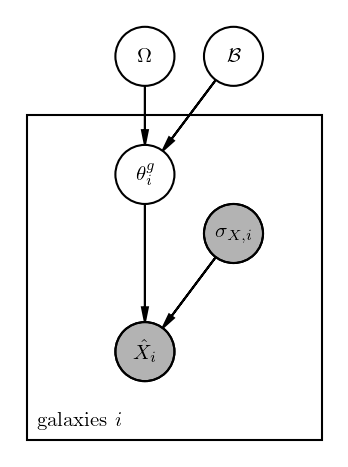
\includegraphics[width=0.4\textwidth]{figs/graph.png} 
    \caption{
    }\label{fig:graph}
\end{center}
\end{figure}



\begin{align}\label{eq:popinf}
p(\Omega, \mathcal{B} \given \{{\bfi X_i}\}) 
    =&~\frac{p(\Omega, \mathcal{B})~p(\{{\bfi X_i}\} \given \Omega, \mathcal{B})}{p(\{{\bfi X_i}\})}\\
    =&~\frac{p(\Omega, \mathcal{B})}{p(\{{\bfi X_i}\})}\int p(\{{\bfi X_i}\}
    \given \{\theta^g_i\})~p(\{\theta^g_i\} \given \Omega, \mathcal{B})~{\rm d}\{\theta^g_i\}.\\
    =&~\frac{p(\Omega, \mathcal{B})}{p(\{{\bfi X_i}\})}\prod\limits_{i=1}^N\int
    p({\bfi X_i} \given \theta^g_i)~p(\theta^g_i \given \Omega, \mathcal{B})~{\rm d}\theta^g_i\\
    =&~\frac{p(\Omega, \mathcal{B})}{p(\{{\bfi X_i}\})}\prod\limits_{i=1}^N\int
    \frac{p(\theta^g_i \given {\bfi X_i})~p({\bfi
    X_i})}{p(\theta^g_i)}~p(\theta^g_i \given \Omega, \mathcal{B})~{\rm d}\theta^g_i\\
    =&~p(\Omega, \mathcal{B})\prod\limits_{i=1}^N\int \frac{p(\theta^g_i \given
    {\bfi X_i})~p(\theta^g_i \given \Omega, \mathcal{B})}{p(\theta^g_i)}~{\rm d}\theta^g_i. 
\intertext{
    We estimate the integral using $S_i$ Monte Carlo samples from the
    individual posteriors $p(\theta^g_i \given {\bfi X_i})$: 
}
    \approx&~p(\Omega, \mathcal{B})\prod\limits_{i=1}^N\frac{1}{S_i}\sum\limits_{j=1}^{S_i}
    \frac{p(\theta^g_{i,j} \given \Omega, \mathcal{B})}{p(\theta^g_{i,j})}.
\end{align} 

